% Section content template for individual Educative lessons
% This file contains the actual content for a specific section
% Generated from Educative API section content

% Section: Class Diagram for Facebook
% Section ID: 4730817050050560
% Section Slug: class-diagram-for-facebook
% Generated: 2025-12-14T12:40:02.891114

In this lesson, we'll identify and design the classes, abstract classes, and interfaces based on the requirements we previously gathered from the interviewer in our Facebook social network system.

\subsection{Components of Facebook}\label{c4Gyr-zsuOPMHGCwzD9y8}
\\
As mentioned, we will design the Facebook social network using a bottom-up approach.

\subsubsection{Person}\label{MaU8M_jGuOX29FKrU1Rt3}
\\
The \texttt{Person} class contains details derived from the \texttt{User} class, such as name, address, phone number, and email.
\\
\paragraph{User}\label{yFUyjA76p6CgtzSVnqP3J}
\\
The \texttt{User} class is Facebook's main class responsible for various operations, such as sending messages or friend requests to other users, creating or joining groups or pages, and numerous others.
\\
The class diagram of these two classes is provided below:
\begin{quote}
\textbf{Note:} The \texttt{User} class contains various methods representing user interactions and functionalities within the system. For brevity, only a subset of these methods is shown here.
\end{quote}

\begin{figure}[htbp]
 \centering
 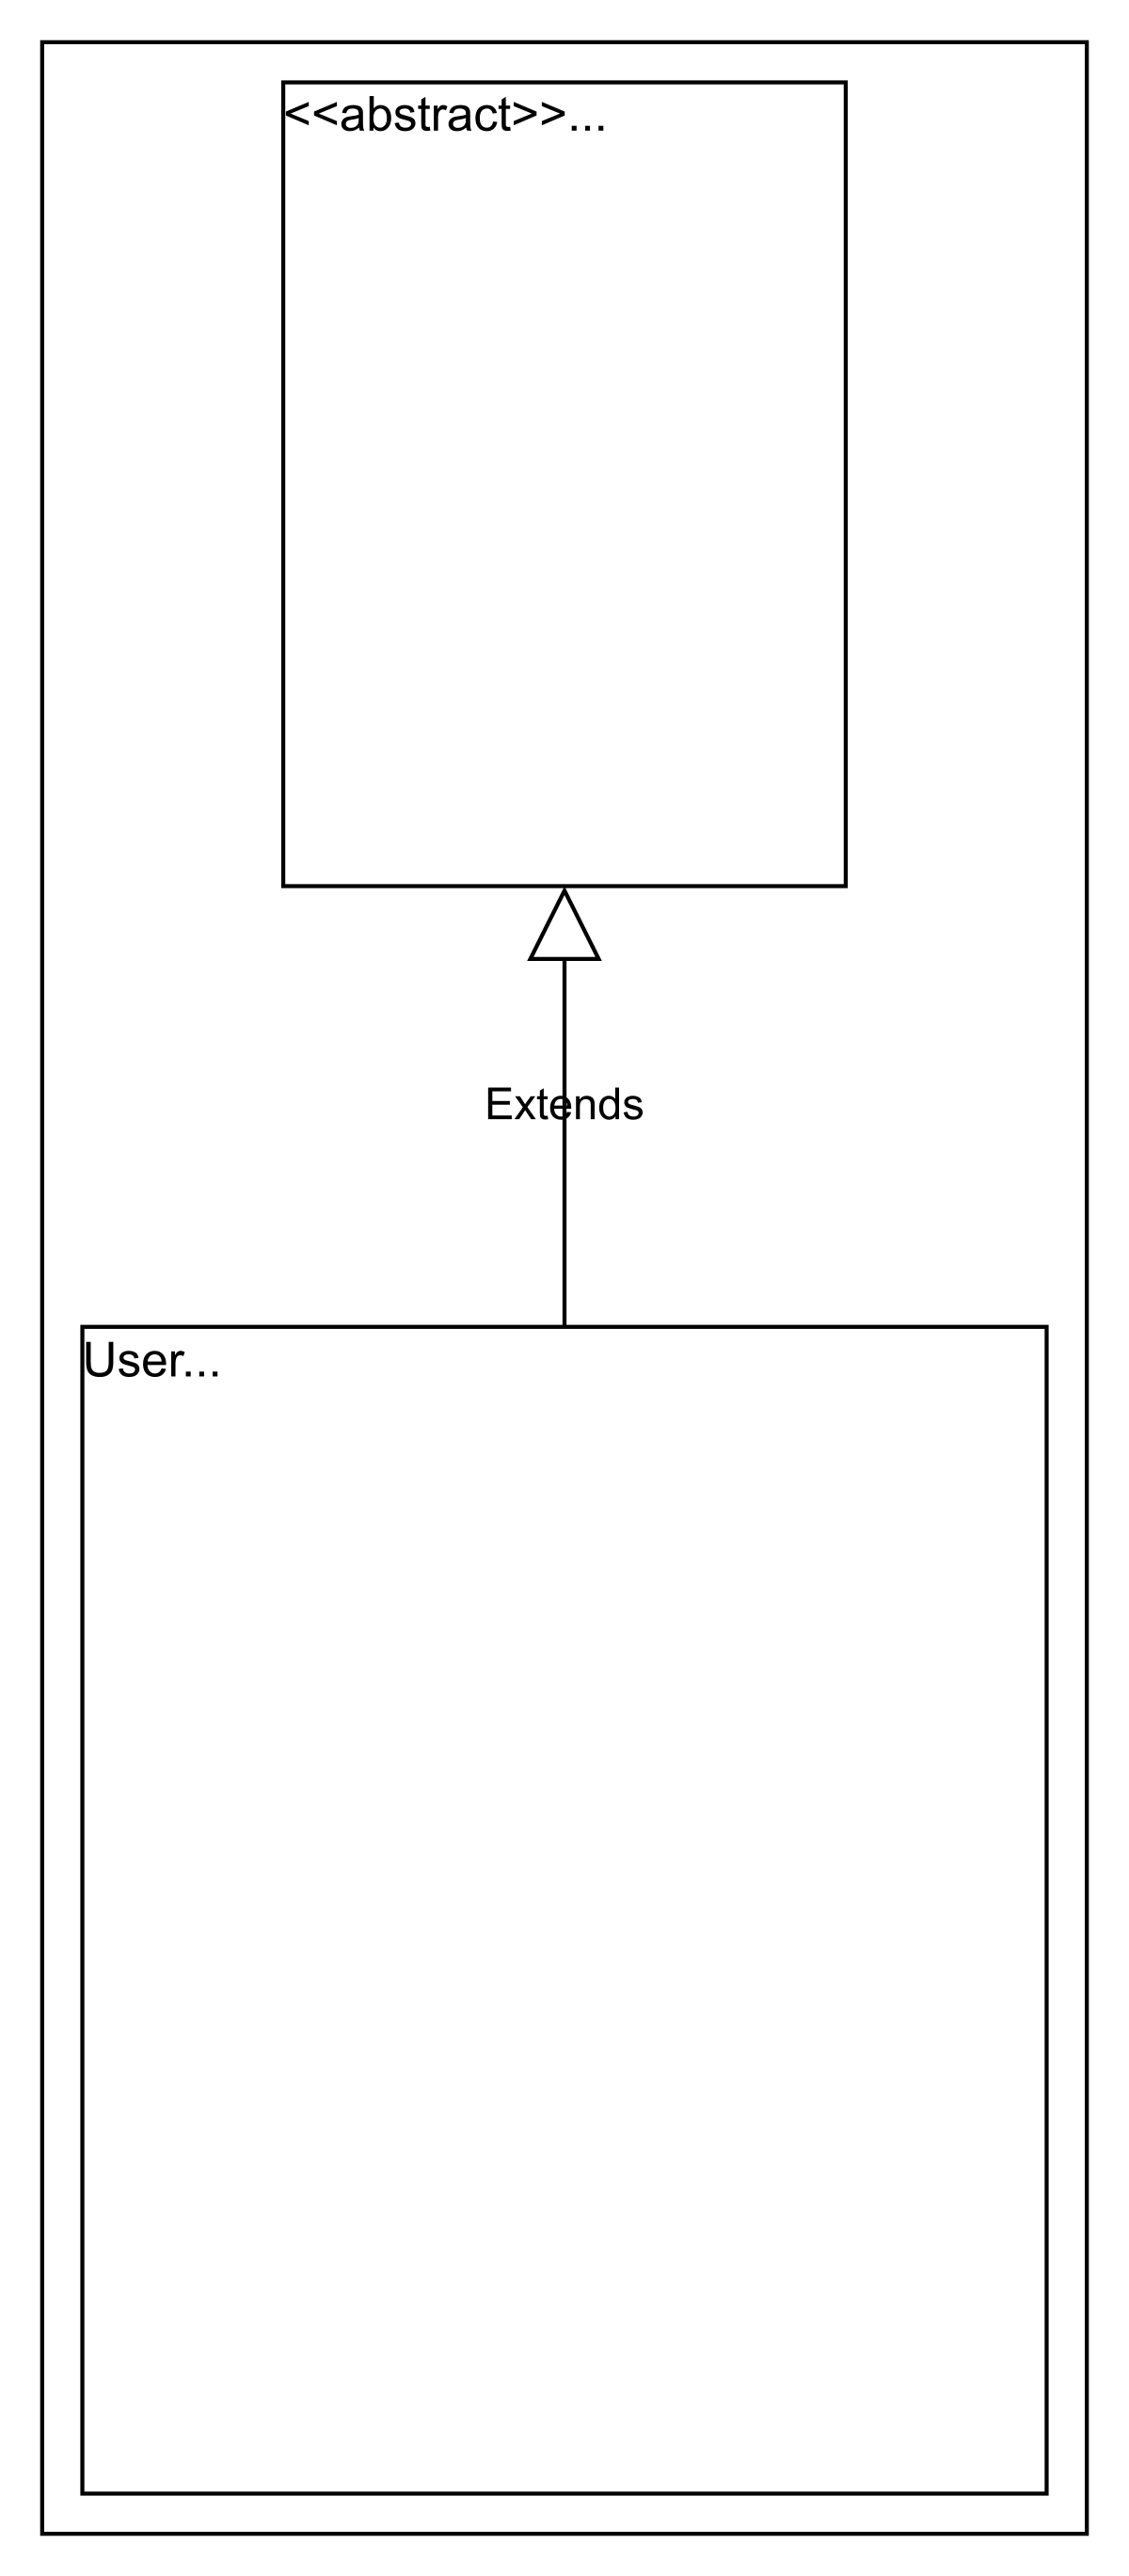
\includegraphics[width=0.5\textwidth]{Images/chapter_22/section_4730817050050560/5172310846603264.png}
 \caption{The class diagram of the Person and User classes}
\end{figure}

\textbf{R4:} Users should be able to send and respond to friend requests, unfriend, and block other users.
\\
\textbf{R8:} A user should be able to send and receive messages from other users.
\\
\textbf{R9:} Users should be able to follow existing pages and join existing groups. They should also be able to unfollow or leave joined groups or followed pages.

\subsubsection{Profile}\label{twppWpSiToBi0EzDEwEhu}
\\
The \texttt{Profile} class contains a Facebook user's personal information, such as their profile and cover pictures, work and education details, and a list of places they've visited.
\\
The visual representation of the \texttt{Profile} class is given below:

\begin{figure}[htbp]
 \centering
 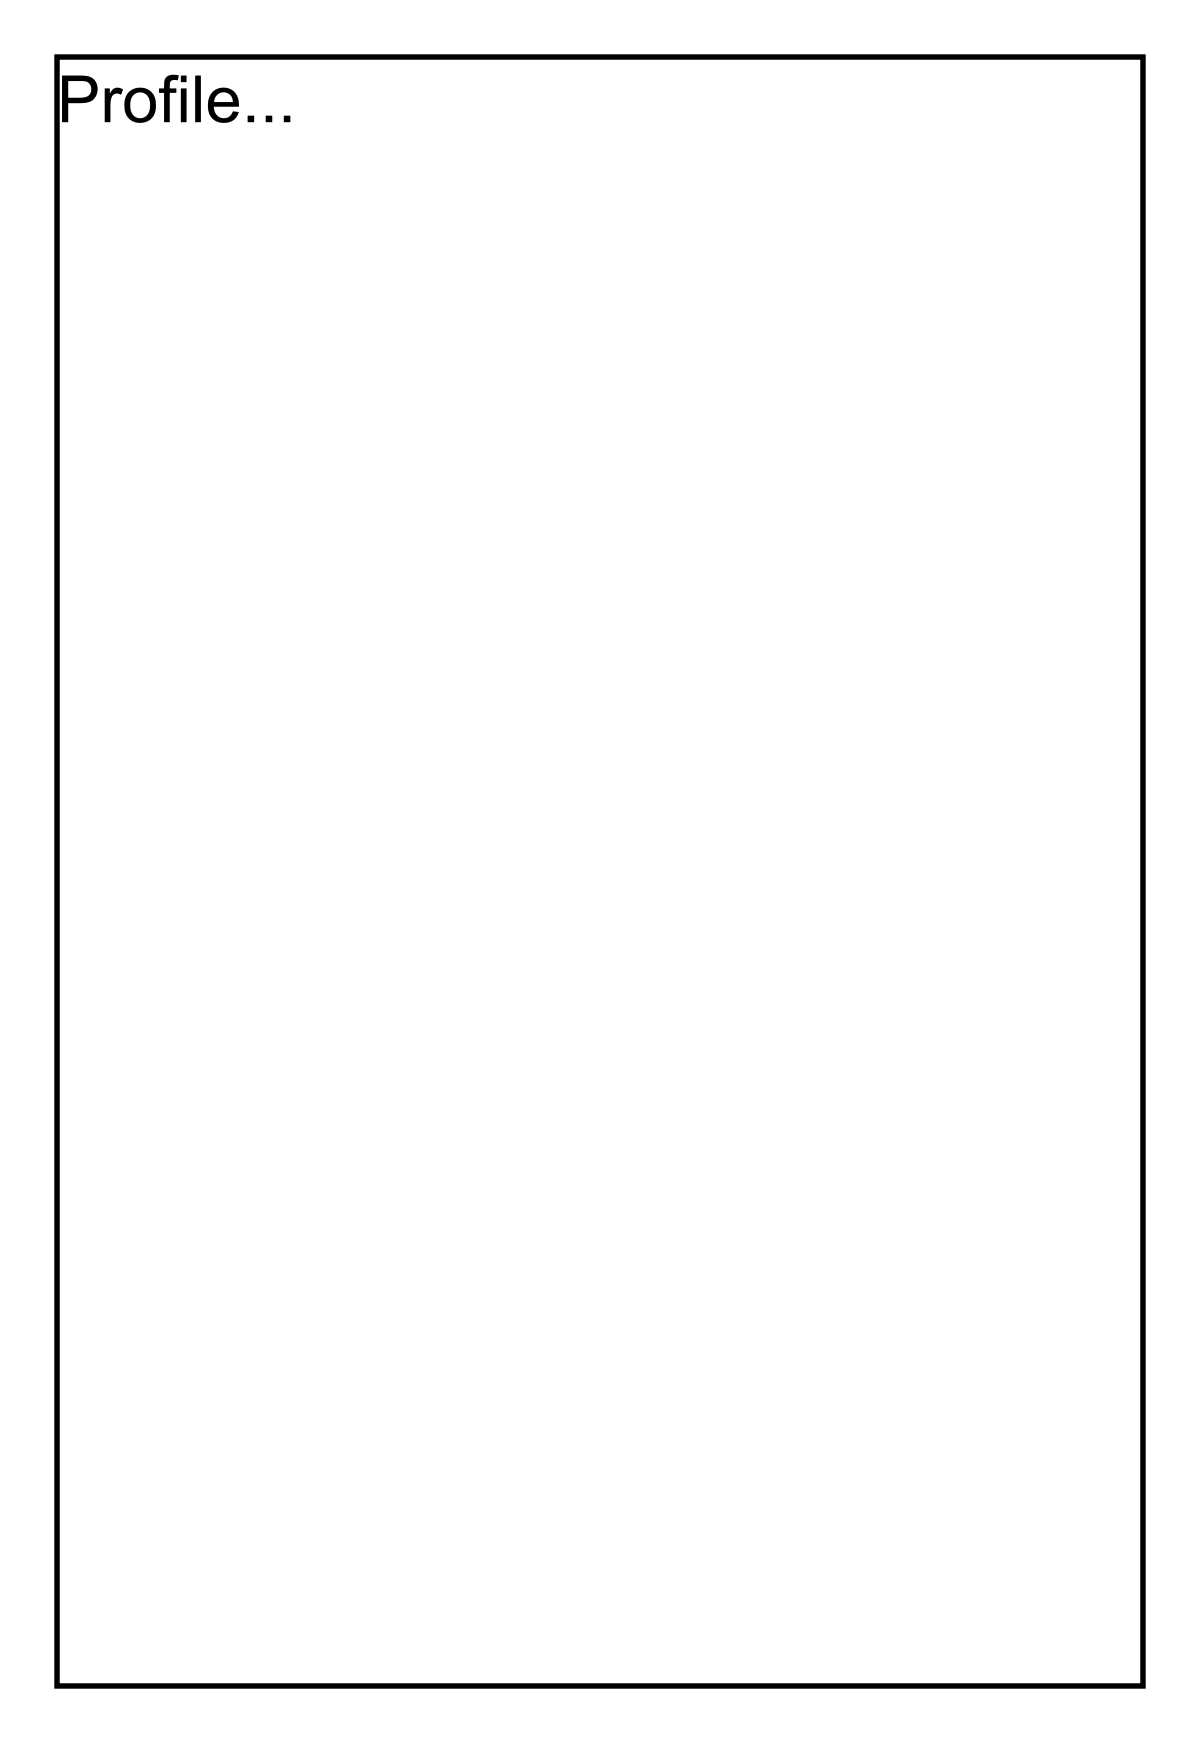
\includegraphics[width=0.5\textwidth]{Images/chapter_22/section_4730817050050560/5492732150546432.png}
 \caption{The class diagram of the Profile class}
\end{figure}

\textbf{R1:} Users should be able to set the privacy of their profile page. They should also be able to create their profile page and add information such as work experience, education, and living place.

\subsubsection{Work, education, and places}\label{hFzZET3RCxEY7x8Pc--ri}
\\
The \texttt{Work}, \texttt{Education}, and \texttt{Places} classes are used to provide relevant information and are involved in the \texttt{Profile} class.
\\
The class representation of these classes is given below:

\begin{figure}[htbp]
 \centering
 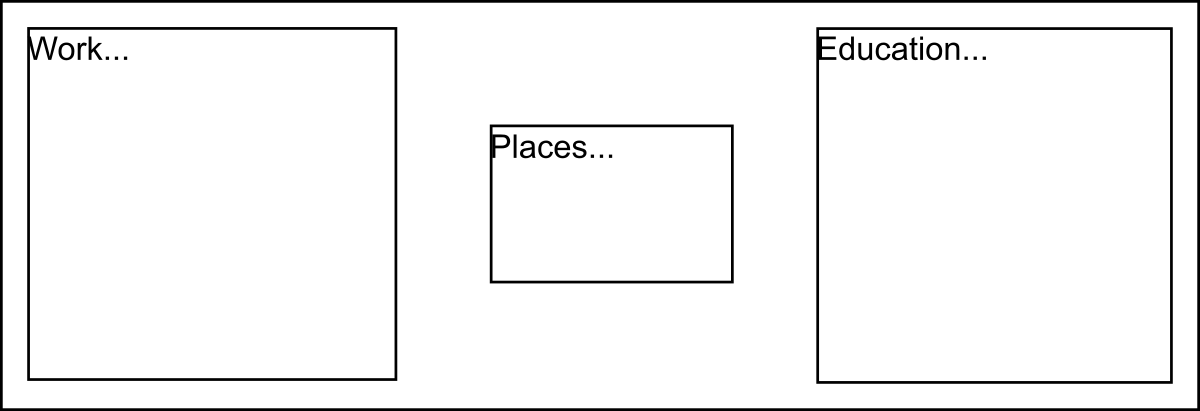
\includegraphics[width=0.5\textwidth]{Images/chapter_22/section_4730817050050560/5015413094350848.png}
 \caption{The class diagram of the Work, Education, and Places classes}
\end{figure}

\textbf{R1:} Users should be able to set the privacy of their profile page. They should also be able to create their profile page and add information such as work experience, education, and living place.

\subsubsection{Page}\label{jxlsCJS3IuU4OE5PDMCpr}
\\
The \texttt{Page} class represents a page on the Facebook platform. It contains the name, description, likes count, and a particular ID to uniquely identify the page.
\\
The UML representation of the class is shown below:

\begin{figure}[htbp]
 \centering
 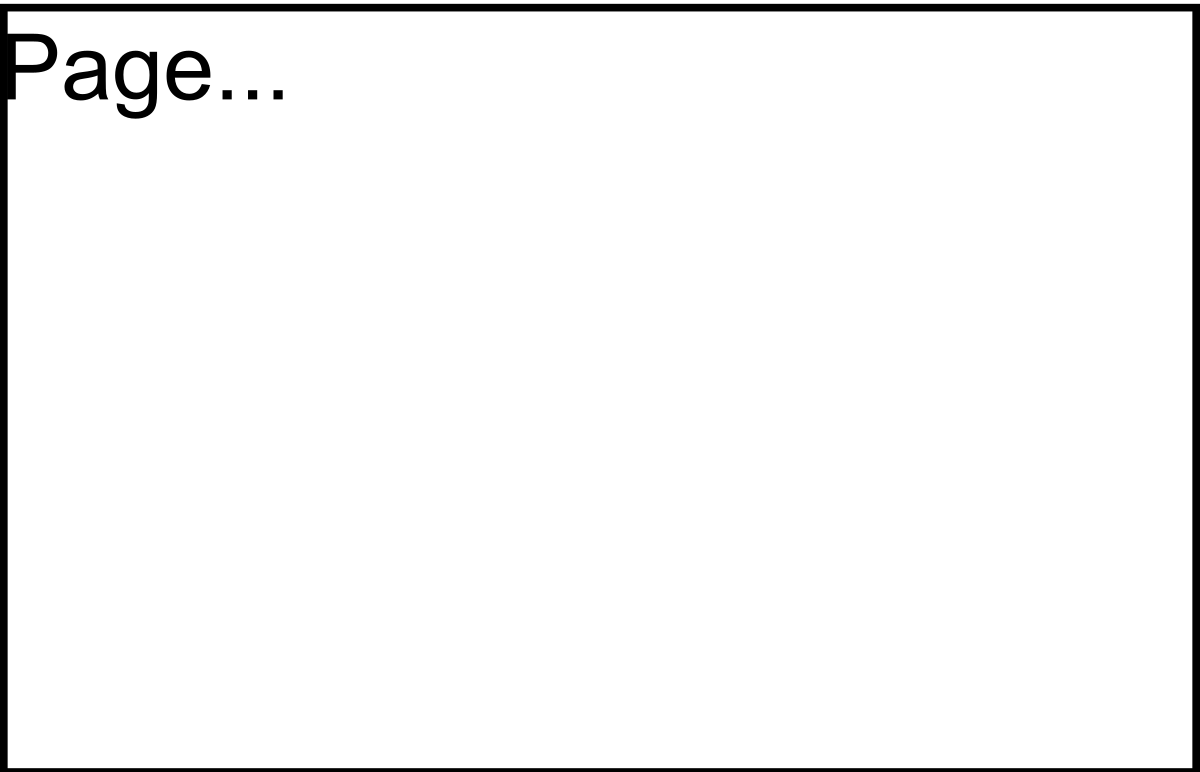
\includegraphics[width=0.5\textwidth]{Images/chapter_22/section_4730817050050560/5597145988333568.png}
 \caption{The class diagram of the Page class}
\end{figure}

\textbf{R9:} Users should be able to follow existing pages and join existing groups. They should also be able to unfollow or leave joined groups or followed pages.

\subsubsection{Group}\label{4EyoCk61xEtyACtKbYo2z}
\\
The \texttt{Group} class represents a particular group on the Facebook platform. It will contain the name, description, total users, and a unique ID to uniquely identify the group. In addition, it will have methods for adding new users and updating the group's description.
\\
The UML representation of the class is shown below:

\begin{figure}[htbp]
 \centering
 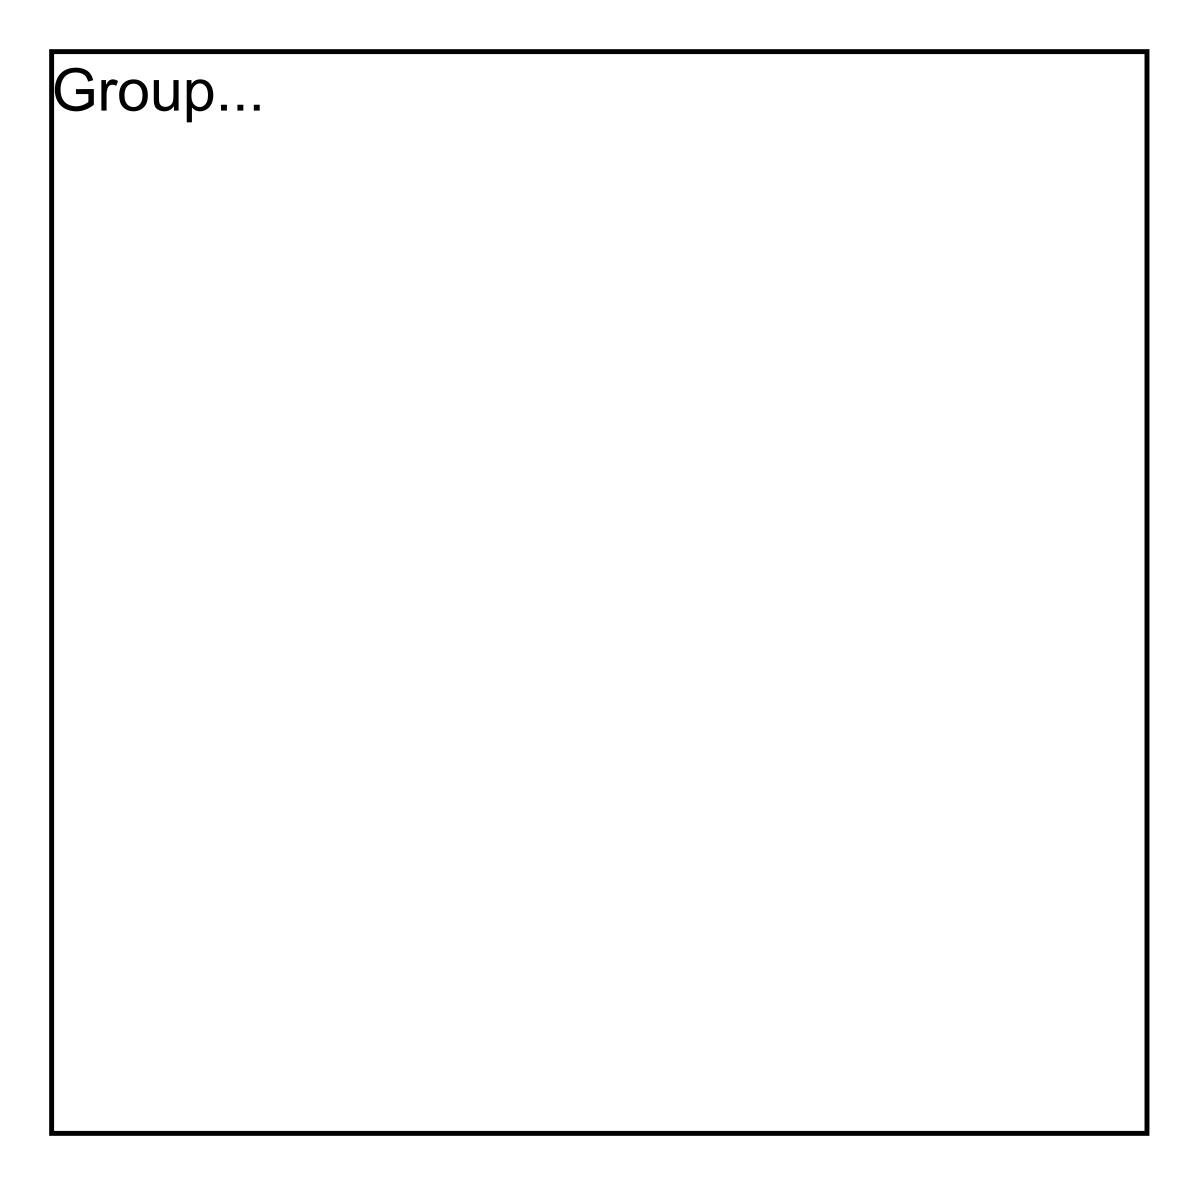
\includegraphics[width=0.5\textwidth]{Images/chapter_22/section_4730817050050560/5527753246769152.png}
 \caption{The class diagram of the Group class}
\end{figure}

\textbf{R9:} Users should be able to follow existing pages and join existing groups. They should also be able to unfollow or leave joined groups or followed pages.

In the Facebook design problem, the \texttt{Group} class implements the \texttt{GroupFunctions} interface.

\begin{figure}[htbp]
 \centering
 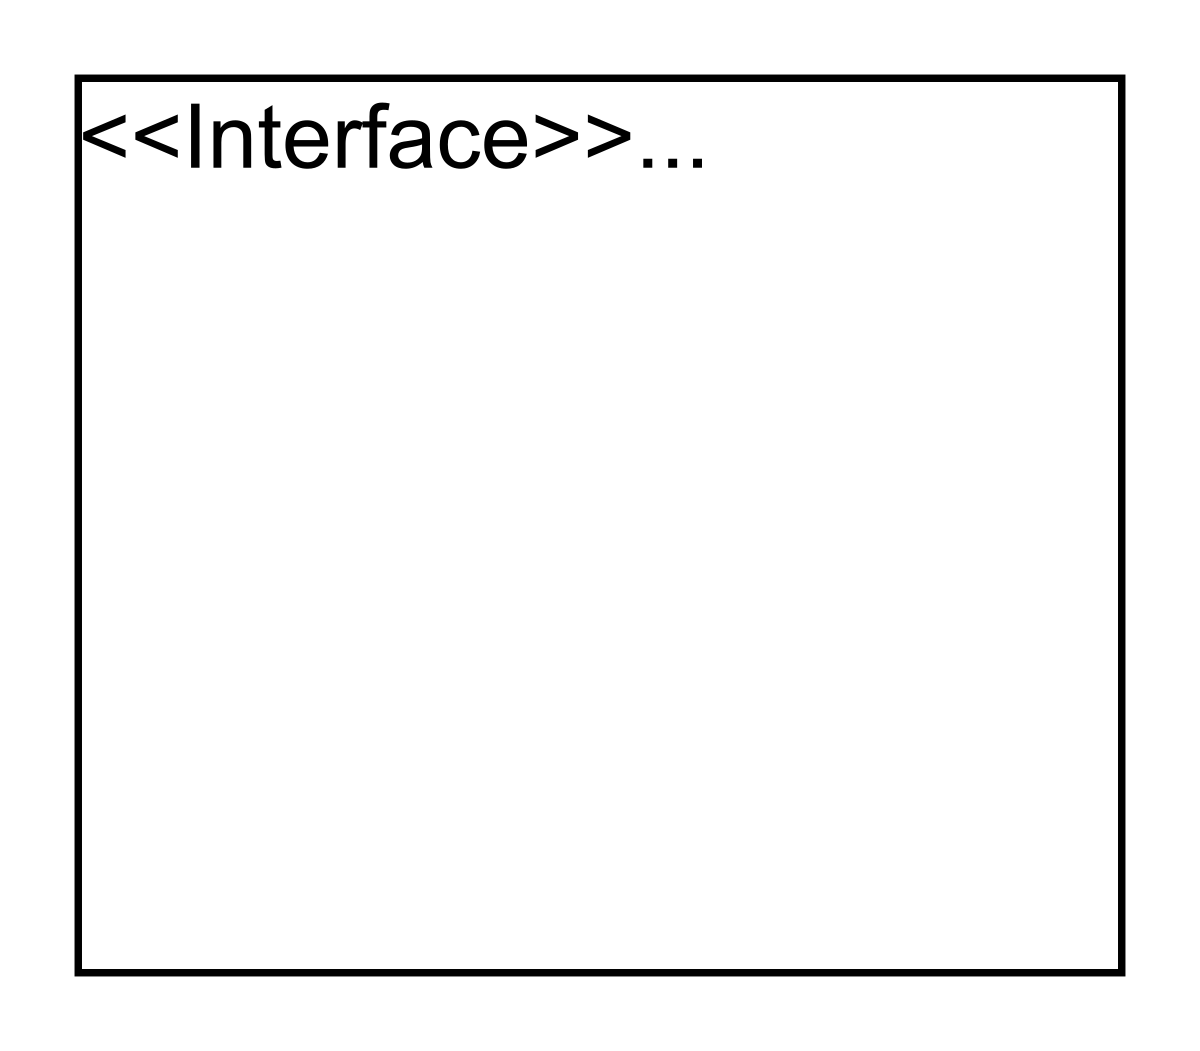
\includegraphics[width=0.5\textwidth]{Images/chapter_22/section_4730817050050560/6653653153611776.png}
 \caption{The GroupFunctions interface as a subscriber}
\end{figure}

\subsubsection{Post}\label{WrXczpeng4hCQI1x1o7qL-2}
\\
The \texttt{Post} class indicates a post by any user that contains its content, the number of likes and shares it has, and its owner. Each post has a specific setting as to who can view it.
\\
The class diagram of the \texttt{Post} class is shown below:

\begin{figure}[htbp]
 \centering
 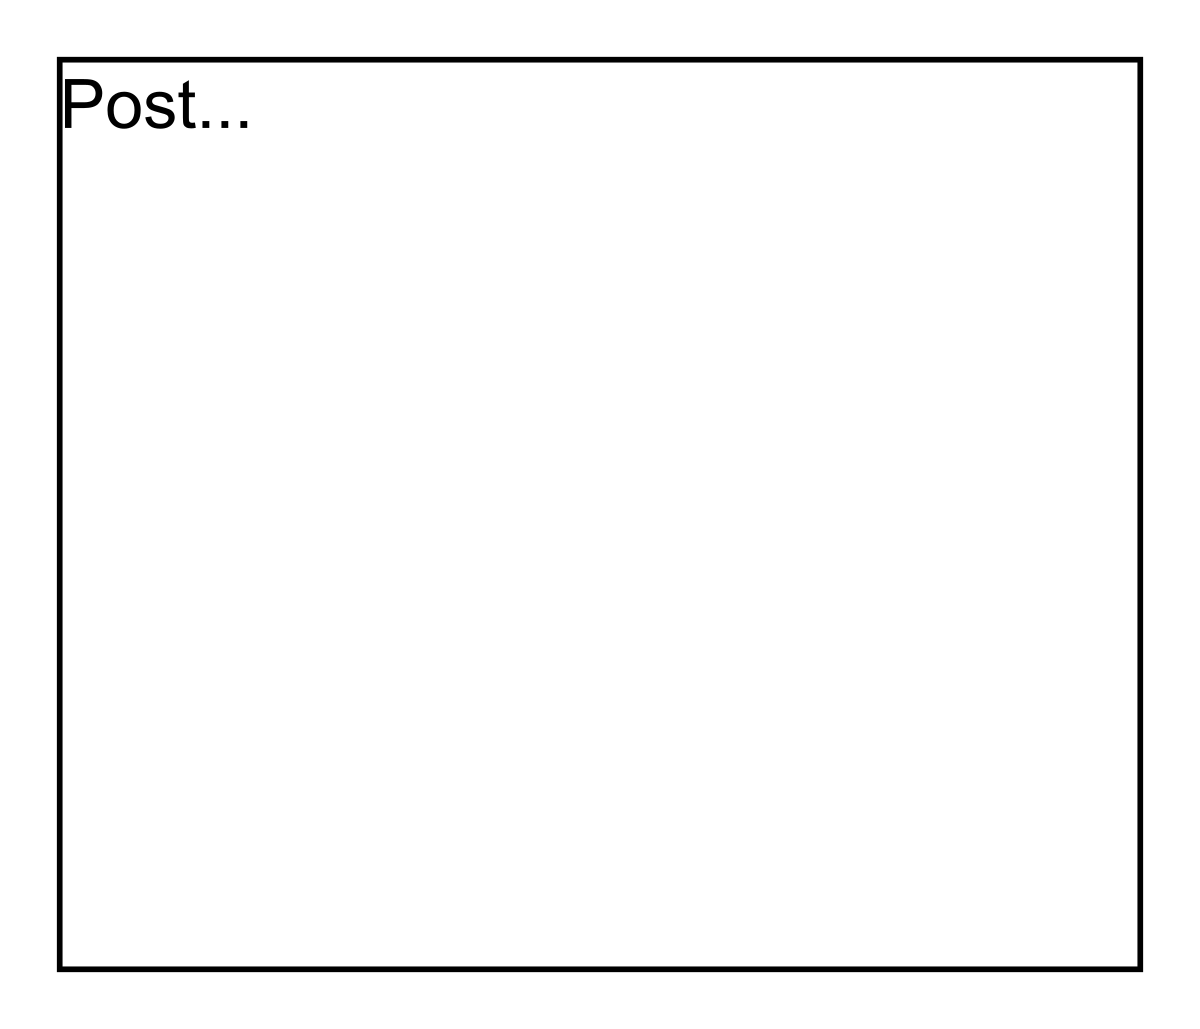
\includegraphics[width=0.5\textwidth]{Images/chapter_22/section_4730817050050560/5533396137541632.png}
 \caption{The class diagram of the Post class}
\end{figure}

\textbf{R3:} Users should be able to write a new post and set its privacy.

\subsubsection{Comment}\label{xBXtMfEwduQ5v67-Sr9aw}
\\
The \texttt{Comment} class indicates a comment by any user on a post that will contain its content, the number of likes, and the owner of the comment.
\\
The class diagram of the \texttt{Comment} class is shown below:

\begin{figure}[htbp]
 \centering
 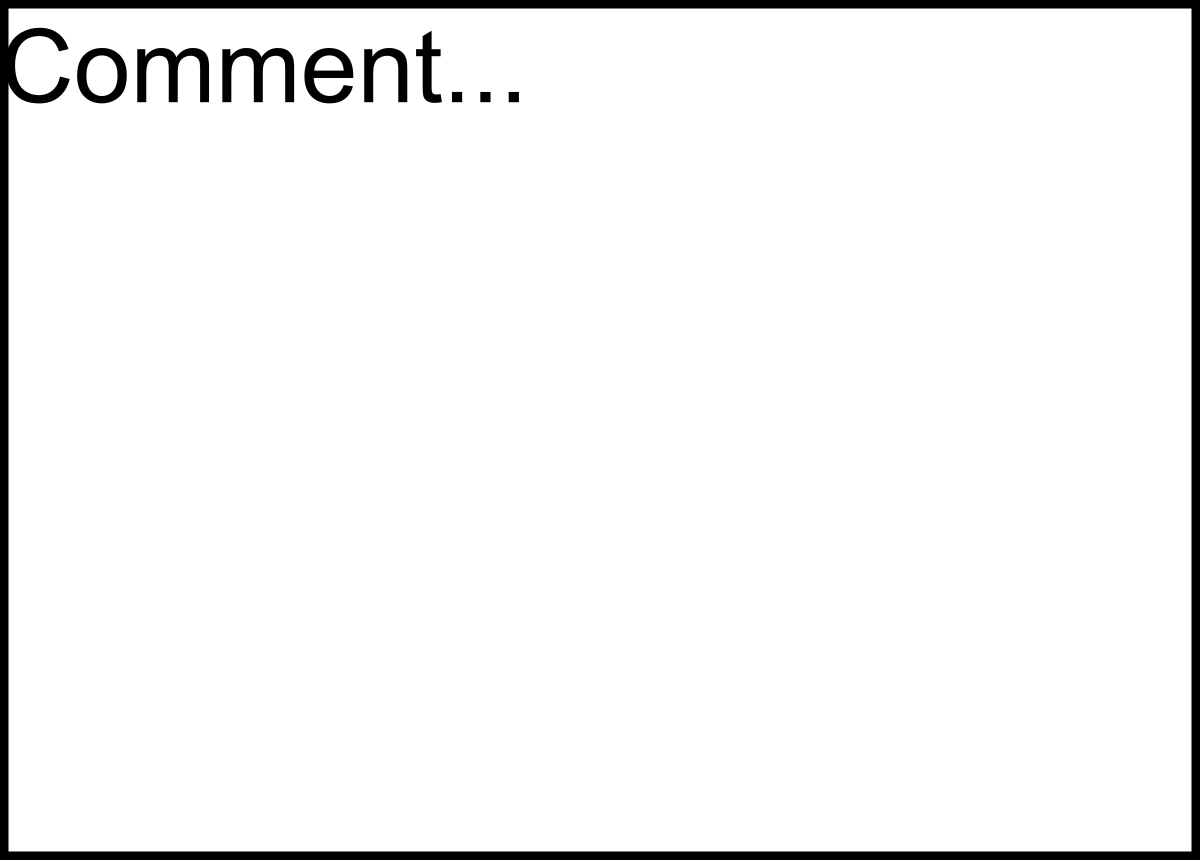
\includegraphics[width=0.5\textwidth]{Images/chapter_22/section_4730817050050560/6051716233691136.png}
 \caption{The class diagram of the Comment class}
\end{figure}

\textbf{R6:} Users should be able to like, share, and/or comment on a post and like or comment on an existing comment.

\subsubsection{Friend request}\label{OzAq7Vny0jcL7yYo0S_KO}
\\
The \texttt{FriendRequest} class describes the details of a friend invitation. It will contain the status of the friend invite and the methods that indicate whether the request was accepted or rejected.
\\
The class diagram of the \texttt{FriendRequest} class is shown below:

\begin{figure}[htbp]
 \centering
 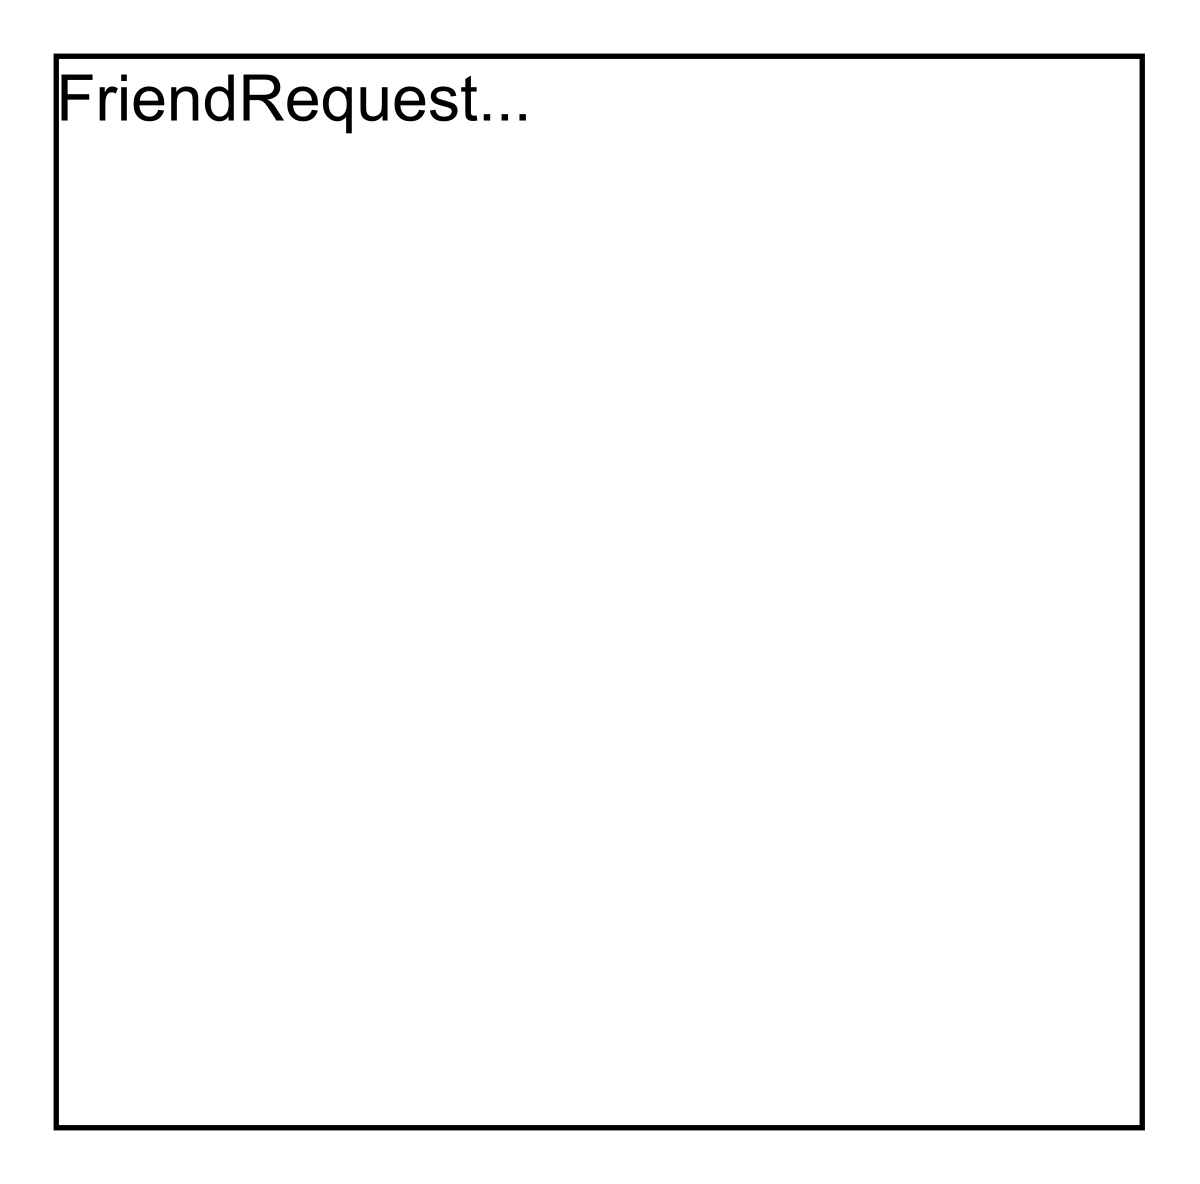
\includegraphics[width=0.5\textwidth]{Images/chapter_22/section_4730817050050560/5086300603285504.png}
 \caption{The class diagram of the FriendRequest class}
\end{figure}

\textbf{R4:} Users should be able to send and respond to other users' friend requests. Users should also be able to unfriend or block other users.

\subsubsection{Message}\label{swkpSyiAJ-FnCDXknDch3}
\\
The \texttt{Message} class represents the message sent by a user to other users.
\\
The class diagram for the \texttt{Message} class is shown below:

\begin{figure}[htbp]
 \centering
 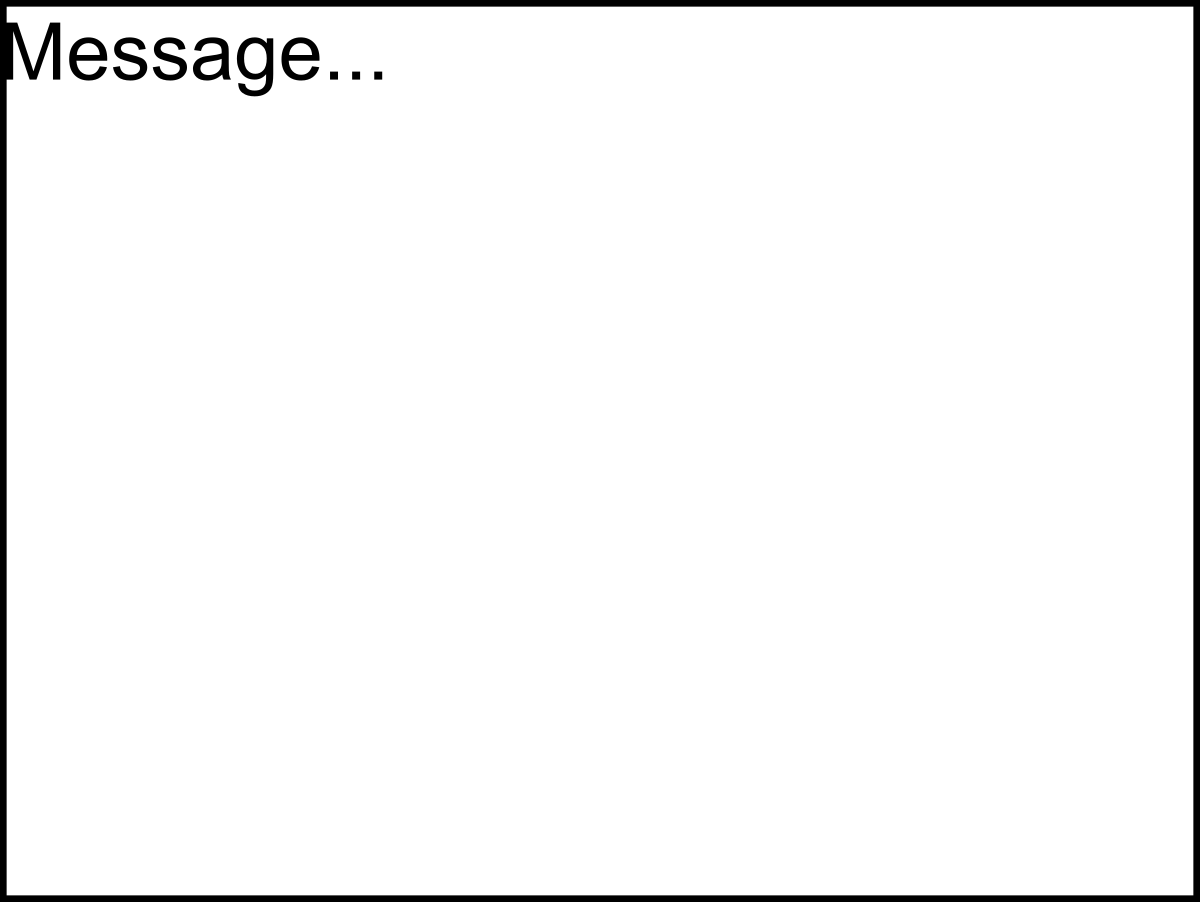
\includegraphics[width=0.5\textwidth]{Images/chapter_22/section_4730817050050560/4764013735182336.png}
 \caption{The class diagram of the Message class}
\end{figure}

\textbf{R8:} A user should be able to send and receive messages from other users.

\subsubsection{Profile privacy}\label{MlNayT3eXgx_koy5dVN0f}
\\
There will be a privacy class for the profile on Facebook. The following represents the class diagram:

\begin{figure}[htbp]
 \centering
 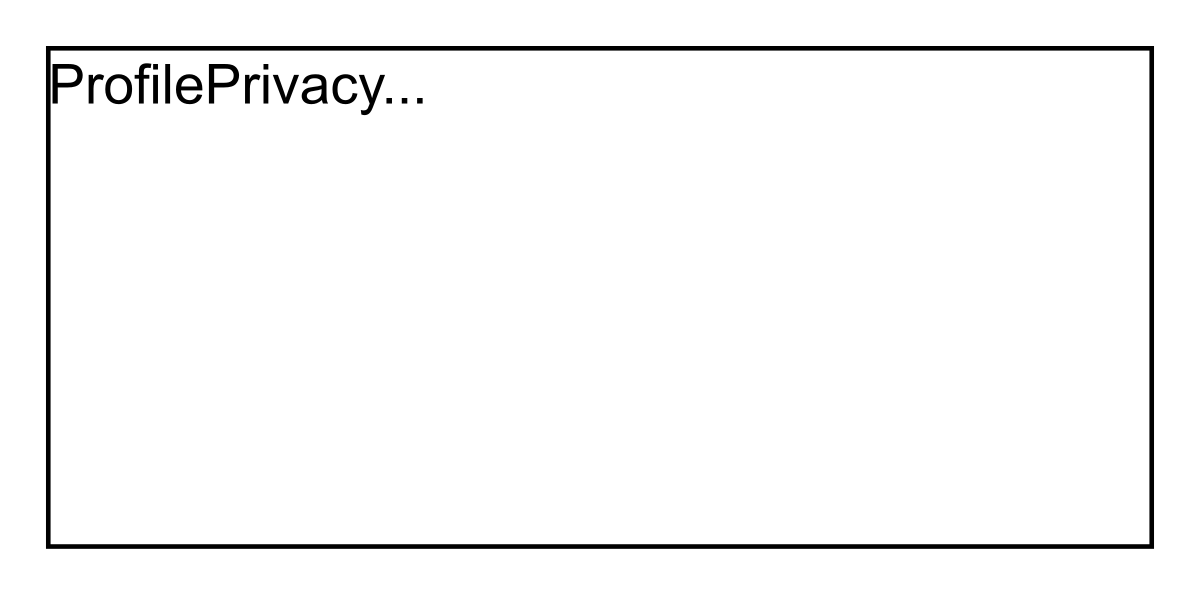
\includegraphics[width=0.5\textwidth]{Images/chapter_22/section_4730817050050560/6182941615849472.png}
 \caption{The class diagram of the ProfilePrivacy class}
\end{figure}

\textbf{R1:} Users should be able to set the privacy of their profile page. They should also be able to create their profile page and add information such as work experience, education, and living place.
\\
\textbf{R3:} Users should be able to write a new post and set its privacy.

\subsubsection{Notification}\label{UhZSkr_T-ji6-tul56ch2}
\\
The \texttt{Notification} class will be a class, since it can send a notification using the built-in notification option. It is mainly responsible for sending notifications whenever any of the following conditions are met:

\begin{itemize}
\item
\protect\phantomsection\label{ZD6Dd0oJFng9C-zSDKUfY}
A friend request is received.
\item
\protect\phantomsection\label{UM2UWuZx3w8qjsAzuE9dx}
A new message is received.
\item
\protect\phantomsection\label{hf6DZNX5jmy6qQURiFLfR}
A new comment is added to a post a user has created or is following.
\item
\protect\phantomsection\label{i4lBxW3rNiQzj6_t8Suq1}
A user has created a new post or a page that another user follows.
\end{itemize}
\\
The UML representation of the class is shown below:

\begin{figure}[htbp]
 \centering
 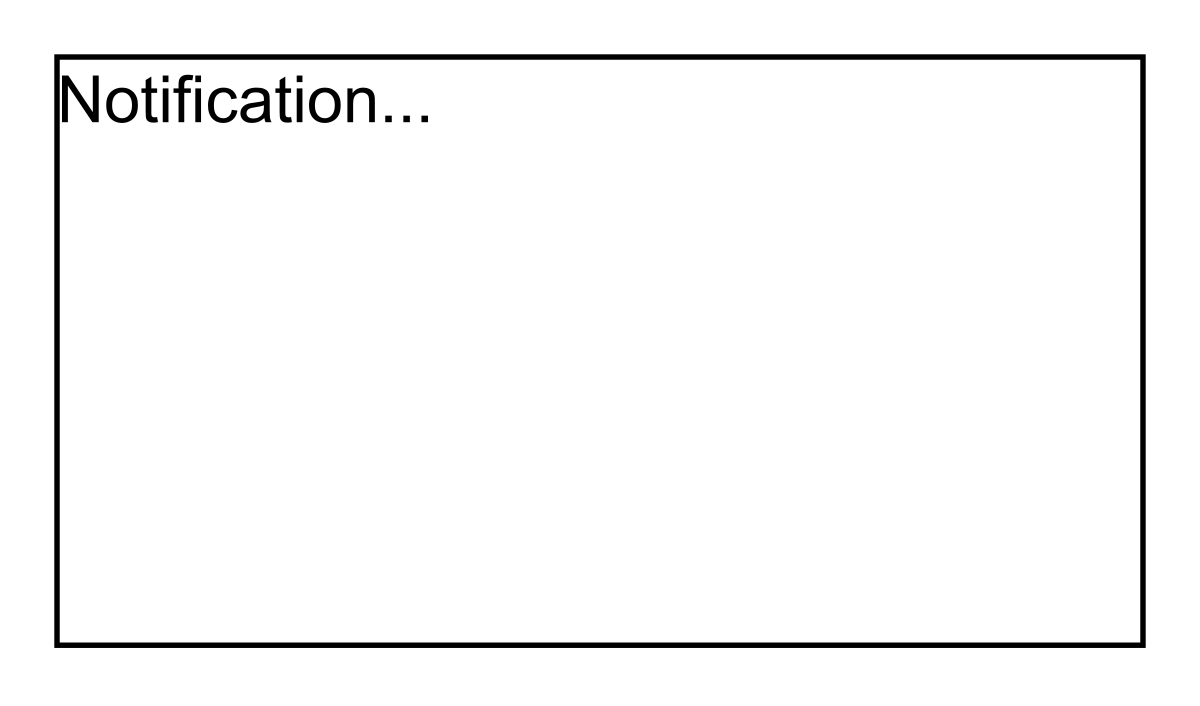
\includegraphics[width=0.5\textwidth]{Images/chapter_22/section_4730817050050560/5309328087973888.png}
 \caption{The class diagram of the Notification class}
\end{figure}

\textbf{R7:} The system should notify the user whenever there has been an interaction with them, such as receiving a message, a friend request, or a comment on their post.

\subsubsection{Interfaces implemented by the user}\label{YDQhuZ6auR1qtkJ9lVyTk}
\\
Several interfaces will exist in the \texttt{Facebook} class, and each will play a separate role in implementing different functionality. The following provides an overview of these:

\begin{itemize}
\item
\protect\phantomsection\label{ldVu5yftwZj6Ylprm0MId}
\texttt{PageFunctionsByUser}\textbf{:} This interface will contain the functions that a user will perform while interacting with pages.
\item
\protect\phantomsection\label{3X-TcGCA4PCjBITpdO53u}
\texttt{GroupFunctionsByUser}\textbf{:} This interface will contain the user's functions while interacting with groups.
\item
\protect\phantomsection\label{wVWnp_VFQ15vtPSOKAmEP}
\texttt{PostFunctionsByUser}\textbf{:} This interface will contain the functions that a user will perform while interacting with posts.
\item
\protect\phantomsection\label{jtb_7FOVizRxuoR67JGOr}
\texttt{CommentFunctionsByUser}\textbf{:} This interface will contain the user's functions while interacting with comments.
\item
\protect\phantomsection\label{loqiY3g-cIqOTuzaL1UOH}
\texttt{Search}\textbf{:} This interface allows customers to search for any particular user, group, page, or post and returns a list of its respective components.
\end{itemize}
\\
The UML representation of the interfaces is shown below:

\begin{figure}[htbp]
 \centering
 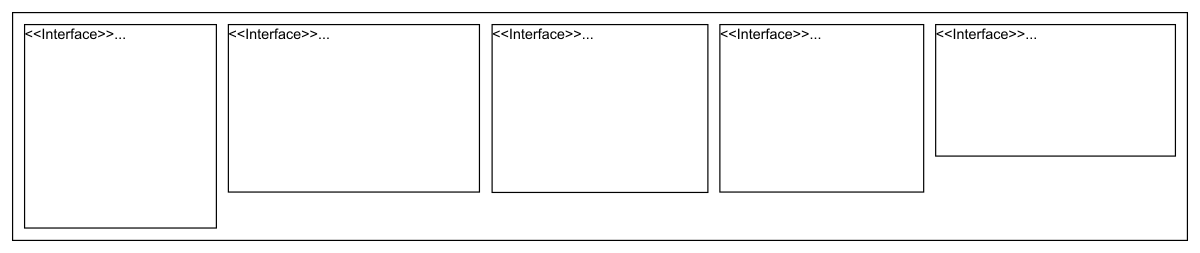
\includegraphics[width=0.5\textwidth]{Images/chapter_22/section_4730817050050560/6384541953294336.png}
 \caption{The class diagram of interfaces to be implemented by users in Facebook}
\end{figure}

\subsubsection{Search catalog}\label{nQm4tZVL6XbCvKn5c7DeE}
\\
\texttt{SearchCatalog} is the class where the search functionality is implemented. Each catalog contains a list of users, groups, pages, and posts, and users can search for users, groups, pages, and posts.
\\
The class representation of the \texttt{SearchCatalog} class is shown below:

\begin{figure}[htbp]
 \centering
 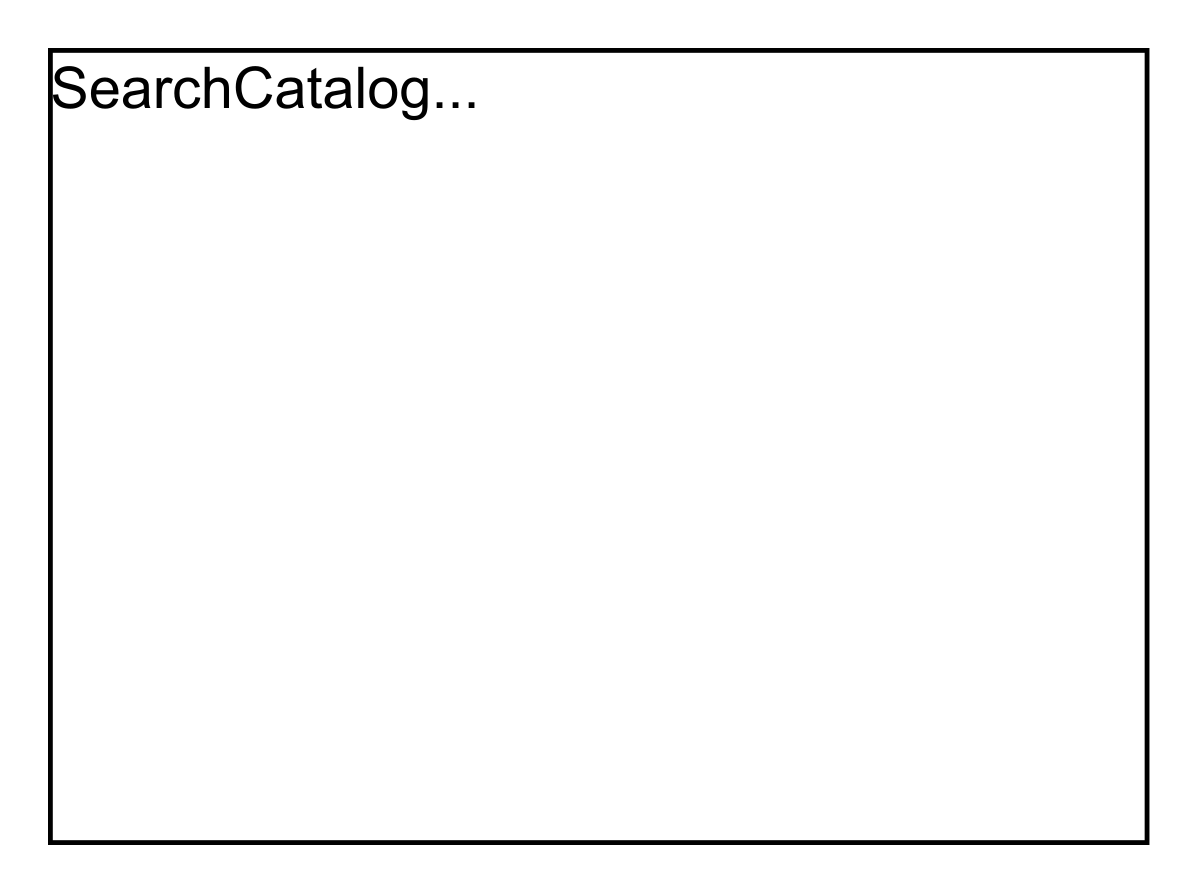
\includegraphics[width=0.5\textwidth]{Images/chapter_22/section_4730817050050560/5812399159246848.png}
 \caption{The class diagram of the SearchCatalog class}
\end{figure}

\textbf{R2:} Our system's users should be able to search for groups, pages, and other users.

\subsubsection{Enumerations}\label{spPUwOm3kRzPiqkKehu98-2}
\\
The enumerations required in the Facebook design are listed below:

\begin{itemize}
\item
\protect\phantomsection\label{txckA_xD4rhwMqhCIiBSN}
\texttt{AccountStatus}\textbf{:} The account status tells about a member's account status, whether it is active, disabled, or blocked.
\item
\protect\phantomsection\label{pNiOVjB8iOsyFFtHGmjJ6}
\texttt{FriendInviteStatus}\textbf{:} The friend invite status describes the status of a friend request, whether it is pending, accepted, rejected, or canceled.
\item
\protect\phantomsection\label{UNbuN-kRaoemVCQRb1GJ1}
\texttt{PostPrivacySettings}\textbf{:} The post-privacy settings enumeration outlines the audience that can view the posts.
\item
\protect\phantomsection\label{UNbuN-kRaoemVCQRb1GJ1}
\texttt{Role}: The role status describes whether the user is a regular user or has administrative permissions.
\end{itemize}

\begin{figure}[htbp]
 \centering
 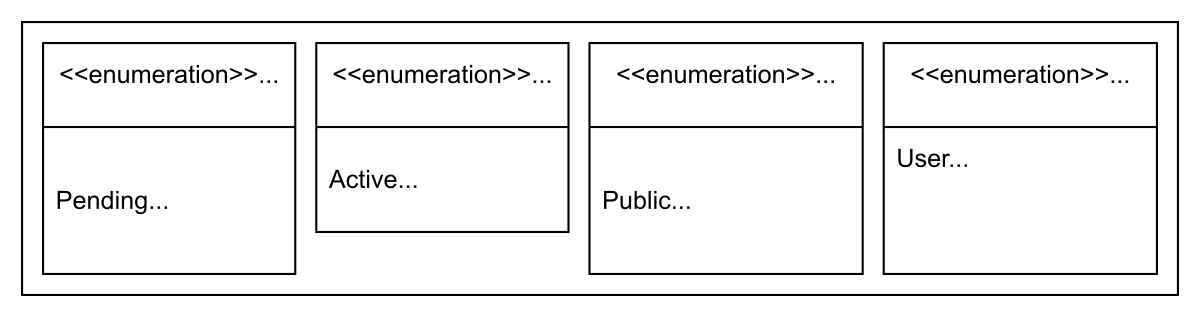
\includegraphics[width=0.5\textwidth]{Images/chapter_22/section_4730817050050560/5419115177967616.png}
 \caption{Enums in Facebook}
\end{figure}

\subsubsection{Custom data type}\label{lwJ49AE-XeLijvqOkj-wl}
\\
We need to create a custom data type, \texttt{Address}, to store a Facebook user's location.

\begin{figure}[htbp]
 \centering
 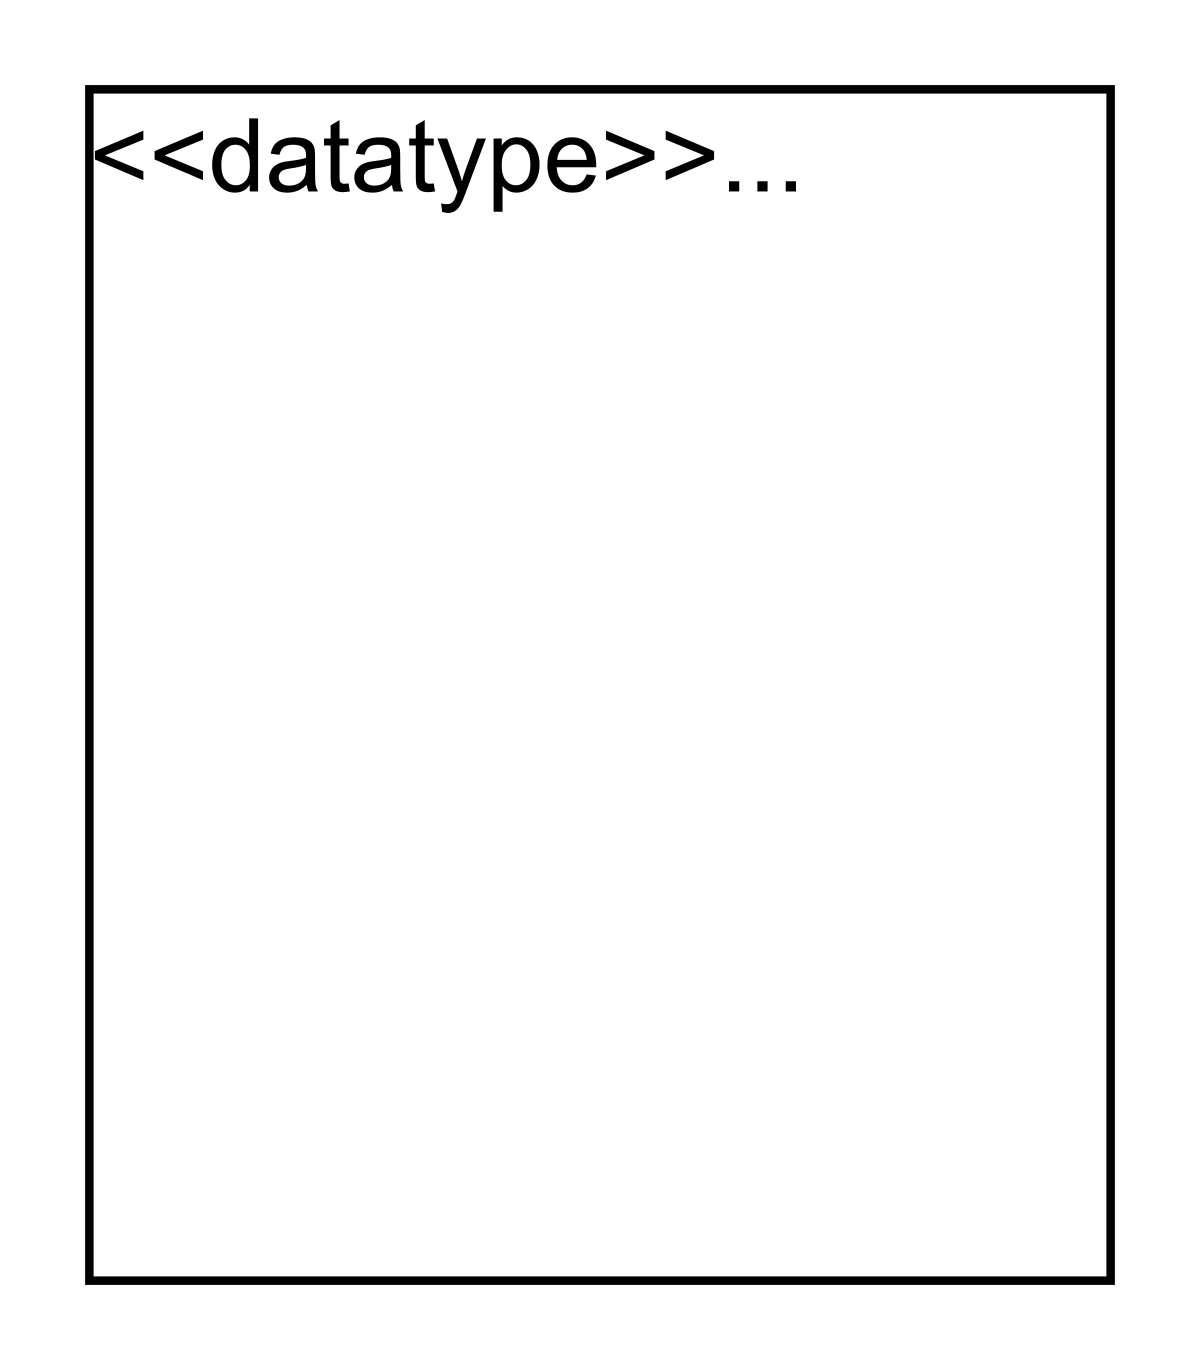
\includegraphics[width=0.5\textwidth]{Images/chapter_22/section_4730817050050560/4884538642530304.png}
 \caption{The class diagram of the custom Address data type}
\end{figure}

\subsection{Relationship between the classes}\label{spPUwOm3kRzPiqkKehu98-3}
\\
Now, we'll discuss the relationships between the classes we have defined above in our Facebook social network system.

\subsubsection{Association}\label{x8qTeRgJ97deskMF9YWD_}
\\
The class diagram has the following association relationships:

\begin{itemize}
\item
\protect\phantomsection\label{DkpUuezwbahlXnqdTZCuS}
The \texttt{User} class has a one-way association with:

\begin{itemize}
\item
Itself
\item
The \texttt{Page}, \texttt{Group}, \texttt{FriendRequest}, \texttt{Message}, \texttt{Comment}, \texttt{Post}, \texttt{ProfilePrivacy}, and \texttt{PostPrivacy} classes.
\item
The \texttt{PageFunctionsByUser}, \texttt{GroupFunctionsByUser}, \texttt{CommentFunctionsByUser}, \texttt{PostFunctionsByUser}, and \texttt{Search} interfaces.
\end{itemize}
\item
\protect\phantomsection\label{tUlAx3mWkHsHKBGmaT2n3}
The \texttt{Profile} class has a one-way association with \texttt{ProfilePrivacy}.
\item
\protect\phantomsection\label{TmgEw_yfkXB5WZB7UHCnx}
The \texttt{Post} class has a one-way association with \texttt{PostPrivacy} and \texttt{Notification}.
\item
\protect\phantomsection\label{F4UnnJlCLmvrB3JUE3F7Q}
The \texttt{Notification} class has a one-way association with \texttt{FriendRequest}, \texttt{Message}, and \texttt{Comment}.
\end{itemize}

\begin{figure}[htbp]
 \centering
 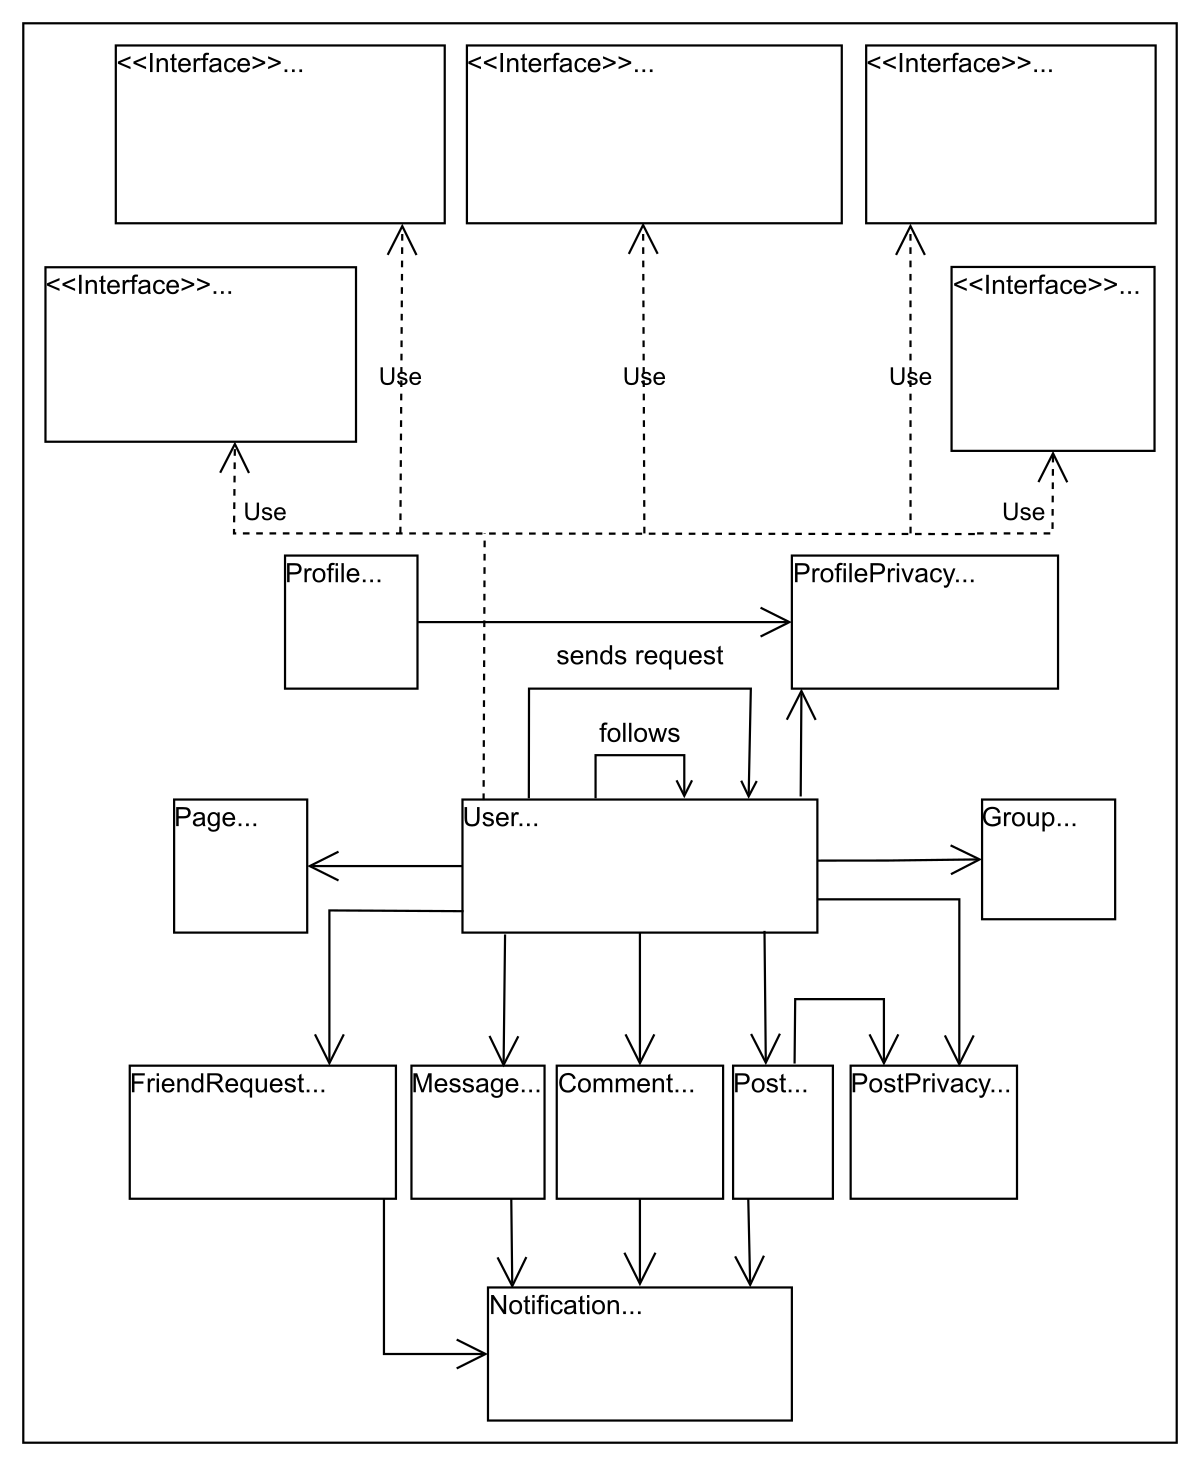
\includegraphics[width=0.5\textwidth]{Images/chapter_22/section_4730817050050560/6748587210702848.png}
 \caption{The association relationship between classes}
\end{figure}

\subsubsection{Composition}\label{spPUwOm3kRzPiqkKehu98-4}
\\
The class diagram has the following composition relationships:

\begin{itemize}
\item
\protect\phantomsection\label{DezRTXoto9k3-XU7e_KiG}
The \texttt{User} class is composed of the \texttt{Profile} class.
\end{itemize}

\begin{figure}[htbp]
 \centering
 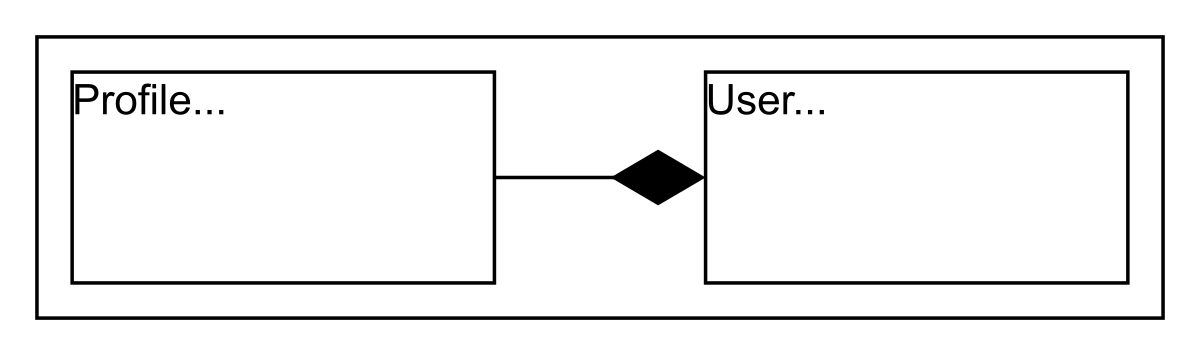
\includegraphics[width=0.5\textwidth]{Images/chapter_22/section_4730817050050560/6262724307582976.png}
 \caption{The composition relationship between classes}
\end{figure}

\subsubsection{Aggregation}\label{TXP5lJqxi6CRl4RPR67M5}
\\
The following classes show an aggregation relationship:

\begin{itemize}
\item
\protect\phantomsection\label{OPSfWe2m7JvywM1Bav-Cu}
The \texttt{Profile} class contains the \texttt{Work}, \texttt{Education}, and \texttt{Places} classes.
\end{itemize}

\begin{figure}[htbp]
 \centering
 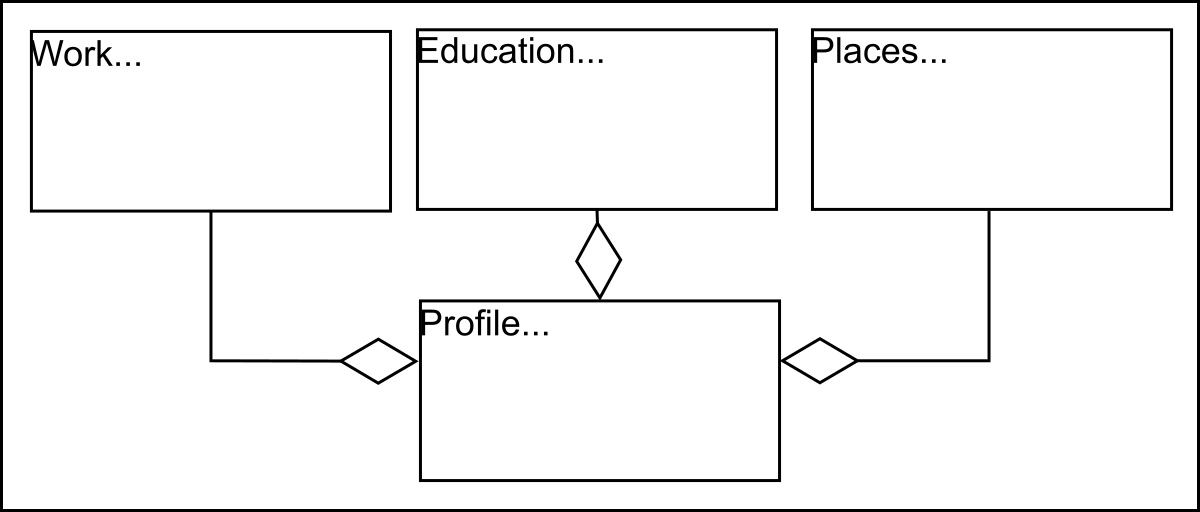
\includegraphics[width=0.5\textwidth]{Images/chapter_22/section_4730817050050560/6144075235590144.png}
 \caption{The aggregation relationship between classes}
\end{figure}

\subsubsection{Generalization}\label{spPUwOm3kRzPiqkKehu98-5}
\\
The following classes show a generalization relationship:

\begin{itemize}
\item
\protect\phantomsection\label{tIhXE_Qw-O6jyfJHeaqWA}
The \texttt{SearchCatalog} class implements the \texttt{Search} interface.
\item
\protect\phantomsection\label{qhNpaMzypMTiu5n14R5Vd}
The \texttt{Group} class implements the \texttt{GroupFunctions} interface.
\end{itemize}

\begin{figure}[htbp]
 \centering
 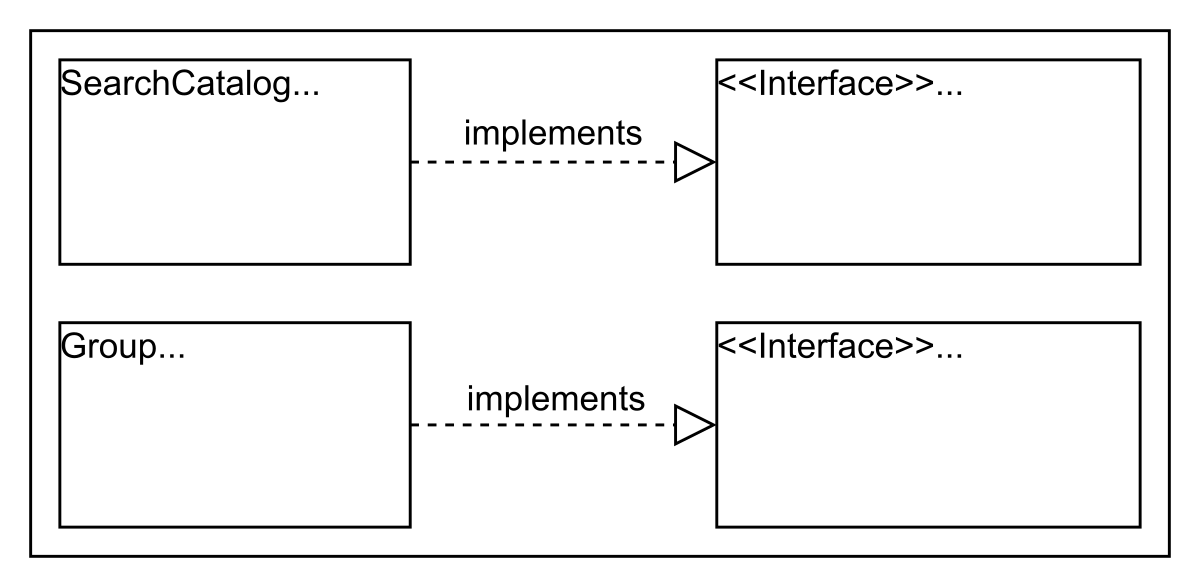
\includegraphics[width=0.5\textwidth]{Images/chapter_22/section_4730817050050560/4928982729228288.png}
 \caption{The generalization relationship between classes}
\end{figure}

\subsubsection{Inheritance}\label{spPUwOm3kRzPiqkKehu98-6}
\\
The following classes show an inheritance relationship:

\begin{itemize}
\item
\protect\phantomsection\label{9jMl5ZP5Fh_1WOZzUklNC}
The \texttt{User} class extends the \texttt{Person} class.
\end{itemize}

\subsection{Class diagram of Facebook}\label{z56aRH_zbEFvqhtCx82ic}
\\
This section outlines the multiplicity (cardinality) relationships between the main classes in our Facebook design system. We explain the allowed number of instances on each side for each relationship and the real-world or design rationale behind the connection. Understanding these relationships is key to modeling how different entities interact and collaborate to support key workflows in the system.

\begin{table}[h!]
\centering
\begin{tabularx}{\textwidth}{|X|X|X|X|}
\hline
\textbf{Source} & \textbf{Target} & \textbf{Multiplicity} & \textbf{Reason} \\
\hline
User & Post & 1 – 0..* & A user can create, like, share, and comment on multiple posts. \\
\hline
Post & User & 1 – 1 & Each post is associated with exactly one user. \\
\hline
User & Comment & 1 – 0..* & A user can create and interact with multiple comments. \\
\hline
User & Message & 1 – 0..* & A user can create and interact with multiple messages. \\
\hline
User & FriendRequest & 1 – 0..* & A user can create and interact with multiple friend requests. \\
\hline
User & Notification & 1 – 0..* & A user can receive multiple notifications. \\
\hline
FriendRequest & User & 1 – 2 & Friend requests involve two users (sender and recipient). \\
\hline
User & Page & 1 – 0..* & A user can follow, like, or share multiple pages. \\
\hline
User & Group & 1 – 0..* & A user can join or manage several groups. \\
\hline
User & Profile & 1 – 1 & Each user is associated with exactly one profile. \\
\hline
Profile & Work & 1 – 0..* & A profile may include multiple work entries. \\
\hline
Profile & Education & 1 – 0..* & A profile may include multiple education entries. \\
\hline
Profile & Places & 1 – 0..* & A profile may include multiple place entries. \\
\hline
Profile & ProfilePrivacy & 0..1 – 1 & Profile may optionally be linked to a privacy setting. \\
\hline
Group & User & 1 – 1..* & A group consists of one or more users as members. \\
\hline
Page & User & 1 – 1..* & At least one user manages a page. \\
\hline
User & Group, Page & 1 – 0..* & Users can participate in multiple groups and pages. \\
\hline
SearchCatalog & User, Group, Page, Post & 1 – 0..* & Maps searchable terms to multiple corresponding objects. \\
\hline
\end{tabularx}
\caption{Social Media System Entity Relationships}
\label{tab:social_media_relationships}
\end{table}

Here's the complete class diagram for Facebook:

\begin{figure}[htbp]
 \centering
 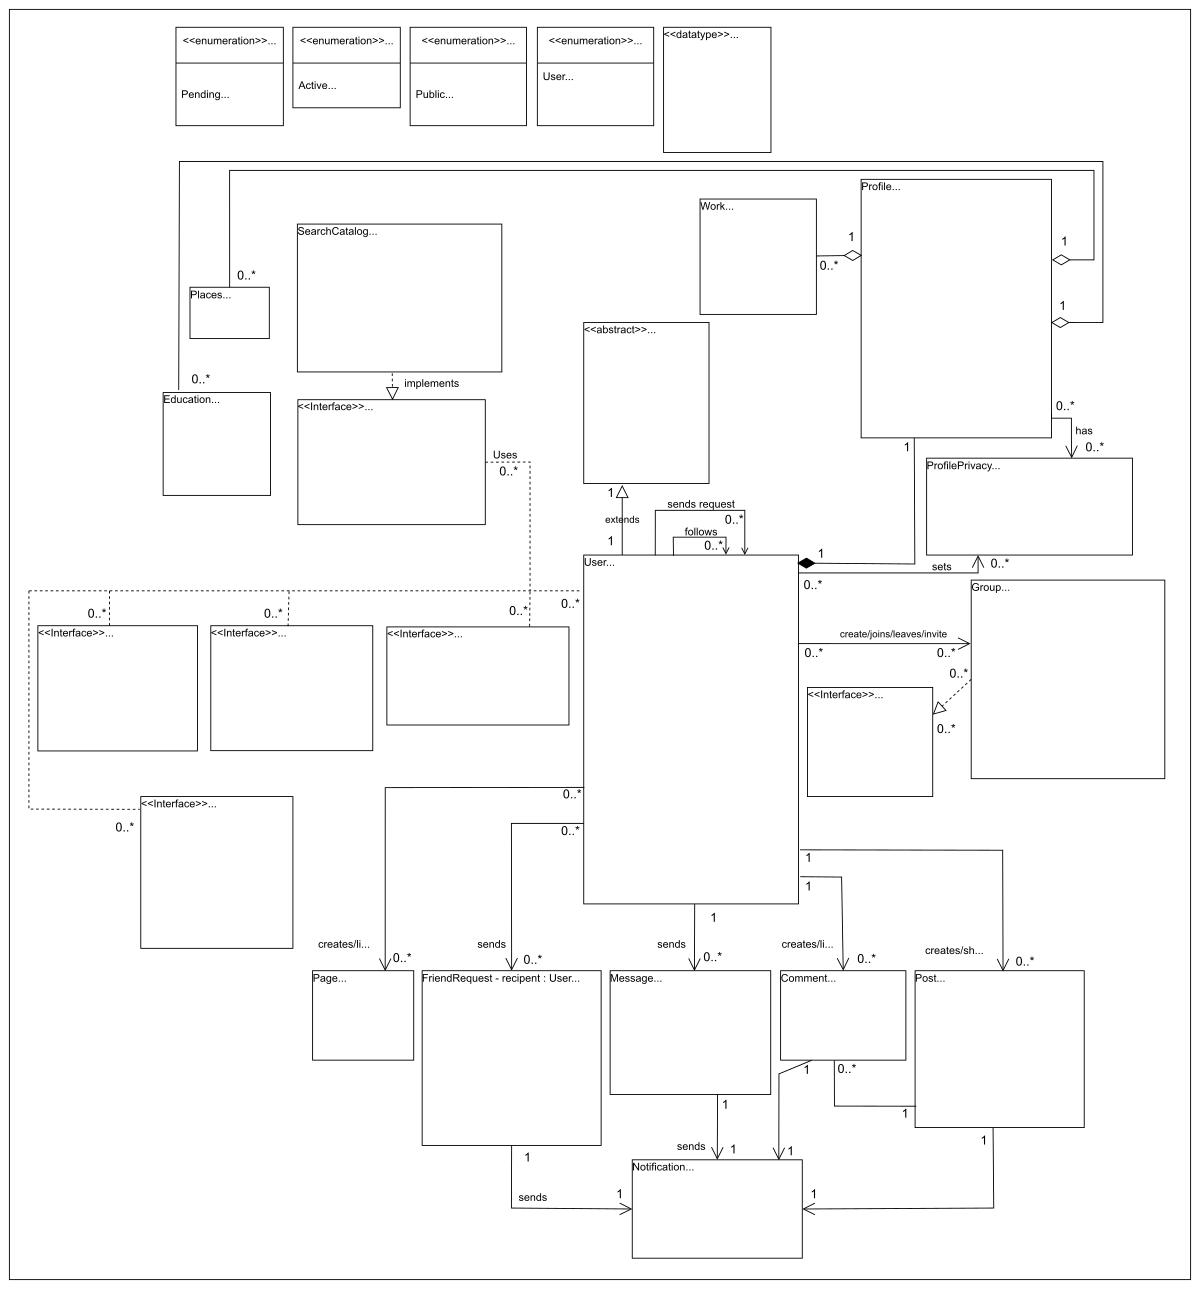
\includegraphics[width=0.5\textwidth]{Images/chapter_22/section_4730817050050560/4773237031305216.png}
 \caption{The class diagram of Facebook}
\end{figure}

\subsection{Design pattern}\label{To1Rbg0qxg88pv77UWZm4}
\\
We apply object-oriented design patterns based on system behavior to implement Facebook's core features flexibly and scalable.

\begin{itemize}
\item
\protect\phantomsection\label{-cv_cFEmjdm0gVP6N41Ow}
We know that Facebook notifies users of new posts, comments, or messages. To model this behavior, we can use the Observer design pattern.
\item
\protect\phantomsection\label{h5DLOh4BSLpJmVIi93Z7z}
We know that Facebook allows users to choose different privacy settings for posts and profiles. To handle this, we can use the Strategy design pattern.
\item
\protect\phantomsection\label{PUl8N_3HZ2N-ezFTsoClE}
Facebook sends different types of notifications. The Factory Method design pattern allows us to create these flexibly.
\item
\protect\phantomsection\label{dwATMp5lGqNW_1hz-MG2w}
We know that Facebook uses a global search feature. We can use the Singleton design pattern to ensure a single shared search service.
\item
\protect\phantomsection\label{ZdVAxBIZVgtCzKaeZ8RMZ}
Facebook users interact with many features, such as posts, groups, and pages. The Interface Segregation principle can separate these responsibilities.
\item
\protect\phantomsection\label{pTXzHOkJuNTQoxRzqYgvn}
We know that Facebook handles status changes in friend requests and user accounts. To manage state-specific behavior, we can use the State design pattern.
\end{itemize}

\subsection{AI-powered trainer}\label{gaKVk_m2APdRROZBNpWSi}
\\
At this stage, everything should be clear. If you encounter any confusion or ambiguity, feel free to utilize the interactive AI-enabled widget below to seek clarification. This tool is designed to help you strengthen your understanding of the concepts.

\begin{figure}[htbp]
 \centering
 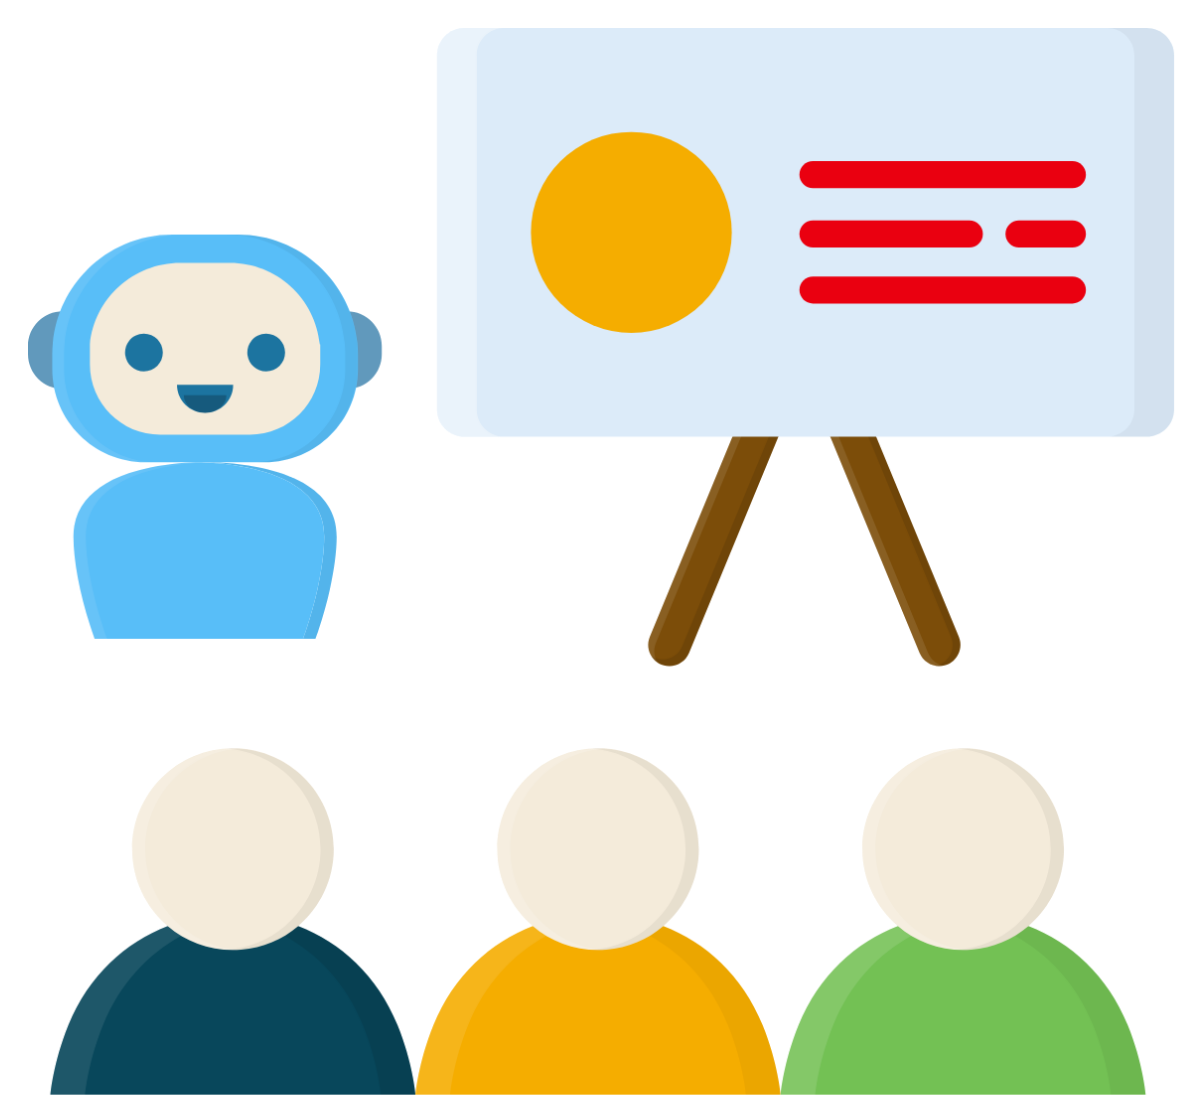
\includegraphics[width=0.15\textwidth]{Images/chapter_22/section_4730817050050560/5047091725205504.png}
 
\end{figure}

\textit{Component type 'PromptAI' not yet supported.}

\subsection{Additional requirements}\label{-f_yjDSmZDAQs8H5k9PlW}
\\
The interviewer can introduce some additional requirements in the Facebook social network system, or they can ask some follow-up questions. Let 's see some examples of additional requirements:

\begin{itemize}
\item
\protect\phantomsection\label{sXSy8ZOuwb1aBt2lZpXYt}
\texttt{Recommendations}\textbf{:} Users can send recommendations of pages and groups to other users. The class diagram provided below shows the relationship of \texttt{Recommendation} with the other classes:
\end{itemize}

\begin{figure}[htbp]
 \centering
 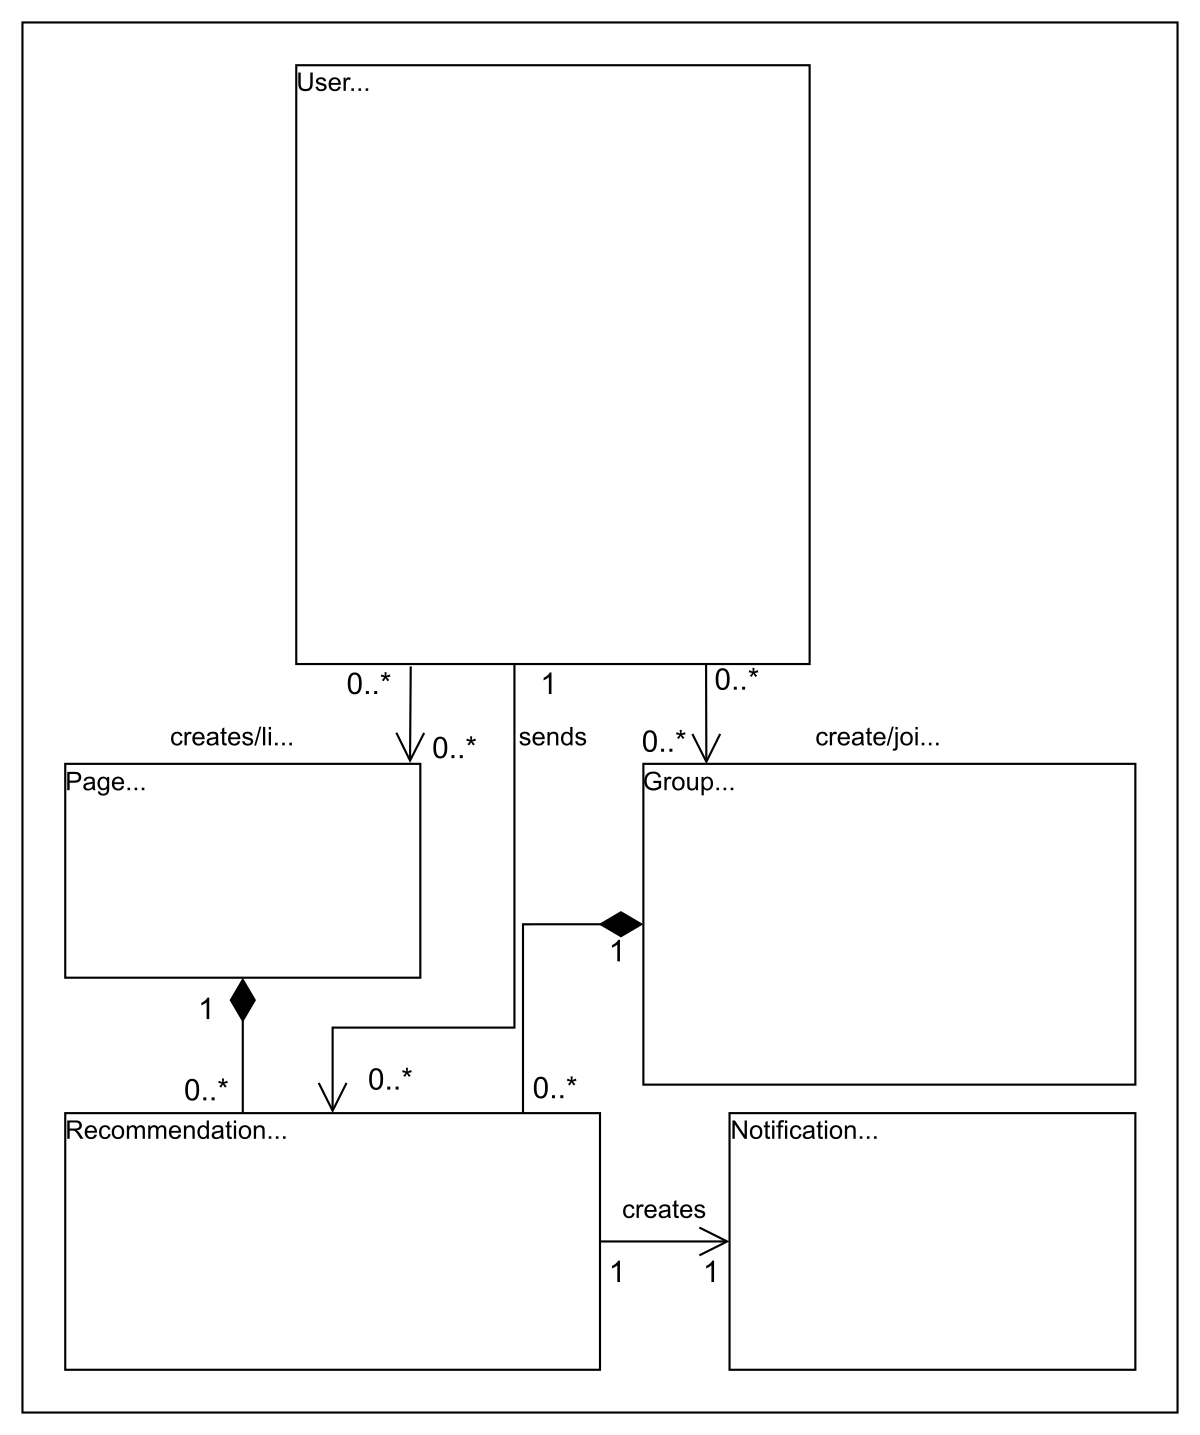
\includegraphics[width=0.5\textwidth]{Images/chapter_22/section_4730817050050560/5973559015768064.png}
 \caption{The class diagram of the Recommendation functionality}
\end{figure}

We have completed the Facebook class diagram according to the requirements. In the next lesson, let's design the Facebook sequence diagram.

% End of section content